\section{Background}
\label{sec:background}
UP-SSO is compatible with OIDC, and achieves the privacy protection based on the SGX.
Here, we provide a brief introduction on OIDC and the SGX.
\subsection{OpenID Connect and PPID}
OIDC~\cite{OpenIDConnect} is an extension of OAuth 2.0 to support user authentication, and has become one of the most prominent SSO authentication protocols. 
Same as other SSO protocols~\cite{SAMLIdentifier}, OIDC involves three entities, i.e., {\em users}, the {\em identity provider (IdP)}, and {\em relying parties (RPs)}.
PPID is suggested in OpenID Connect protocol to protect the user from a possible correlation among RPs.

\vspace{3mm}\noindent\textbf{Implicit flow of user login.}
OIDC supports three processes for the SSO authentication session, known as {\em implicit flow}, {\em authorization code flow} and {\em hybrid flow} (i.e., a mix-up of the previous two). Here, we choose the OIDC implicit flow as the example to illustrate the protocol. 
In the implicit flow, an {\em id token} is generated as the identity proof, which contains a user identifier, an RP identifier, IdP's identifier, the validity period, and other requested attributes.
The IdP signs the id token using its private key to ensure integrity.

\begin{figure}[t]
  \centering
  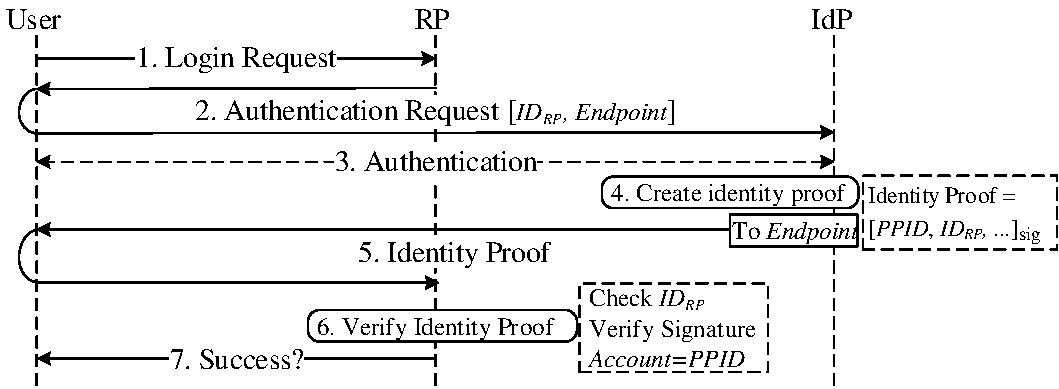
\includegraphics[width=\linewidth]{fig/OIDC1.pdf}
  \caption{The implicit protocol flow of OIDC.}
  \label{fig:OpenID}
\end{figure}

As shown in Figure~\ref{fig:OpenID}, the implicit flow of OIDC consists of 7 steps.
\begin{itemize}
\item[1] At the beginning, user attempts to log in to an RP.
\item[2] RP constructs a request for identity proof, which is redirected by the user to the corresponding IdP. The request contains $ID_{RP}$, RP's endpoint and a set of requested user attributes.
\item[3] If the user has not been authenticated yet, the IdP performs an authentication process.
\item[4] If the RP's endpoint in the request matches the one registered at the IdP, it generates an identity token. Otherwise, IdP generates a warning to notify the user about potential identity proof leakage.
\item[5] IdP sends the identity token back to the RP.
\item[6] The RP verifies the id token, and extracts user identifier from the identity token.
\item[7] Finally, RP returns the authentication result to the user.
\end{itemize}

\vspace{3mm}\noindent\textbf{Pairwise Pseudonymous Identifier (PPID).} 
PPID is the user identifier provided by IdP for RP identifying a user. Different from the normal user ID, PPID is an RP-specific use ID. That is, while a user visits different RPs, IdP would provide different but constant user IDs (i.e., PPID) for these RPs.    
NIST~\cite{NIST2017draft} suggests that PPID should be used to prevent the user's account at the IdP from being easily linked at multiple RPs through use of a common identifier. 
It also suggests that PPID should be either generated randomly and assigned to users by the IdP, or derived from other user's information if the derivation is done in an irreversible, unguessable manner (e.g., using a keyed hash function with a secret key). For example, we have learned that, MITREid Connect~\cite{MITREid}, a popular open source OIDC project, generates PPID using a secure random number generator, and stores the key-value map of corresponding RP and PPID.


\subsection{Intel SGX}
Intel Software Guard Extensions (Intel SGX)~\cite{costan2016intel} is the hardware-based security  mechanism provided by Intel since the sixth generation Intel Core microprocessors. It offers memory encryption that isolates specific application code and data in memory, that allows user-level code to allocate private regions of memory, called enclaves~\cite{costan2016intel}, which guarantees the running code are well protected from the adversary outside the enclave.
 
\vspace{3mm}\noindent\textbf{Enclave.}
The enclave’s code and data is stored in Processor Reserved Memory (PRM). 
PRM is the subset of Dynamic random-access memory (DRAM), and it cannot be directly accessed by other software, including system software and System Management Module code (Ring 2).
The Direct Memory Access (DMA) of PRM is also unavailable, as enclave is protected from other peripherals.



\vspace{3mm}\noindent\textbf{Remote Attestation.} 
Remote attestation~\cite{costan2016intel} enables the software inside an  enclave to attest to a remote entity that it is trusted. That is, during the attestation, the remote entity would receive an SGX attestation signature, containing the enclave’s measurement (a measurement of the code and data loaded in enclave).
The SGX remote attestation allows a player to verify three things, the application's identity, its intactness (that it has not been tampered with), and that it is running securely within an enclave on an Intel SGX enabled platform.
Moreover, with the remote attestation, the secure key exchange between the player and remote enclave application is also available even the application runs in the malicious environment.

 